\subsection{Ring Buffer Based on RDMA and Shared Memory}
\label{socksdirect:subsec:lockless-queue}

\iffalse
\begin{figure}[t]
	\centering
	
\includegraphics[width=0.4\textwidth]{images/fixme.pdf}
	
	\caption{Comparison of queue performance.}
	\label{socksdirect:fig:queue-performance}
\end{figure}
\fi


\begin{figure}[htbp]
	\centering
	\subfloat[Traditional ring buffer.]{
		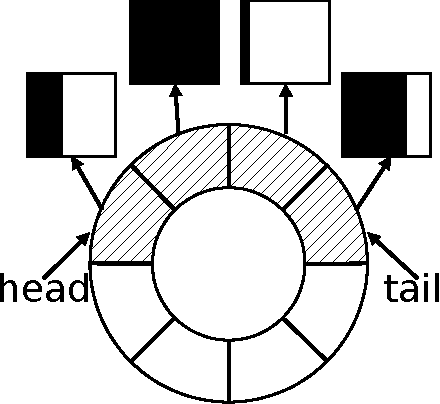
\includegraphics[width=0.3\textwidth]{images/ringbuffer_traditional}
		\label{socksdirect:fig:ringbuffer-traditional}
	}
	\hspace{0.02\textwidth}
	\subfloat[Ring buffer of \sys.]{
		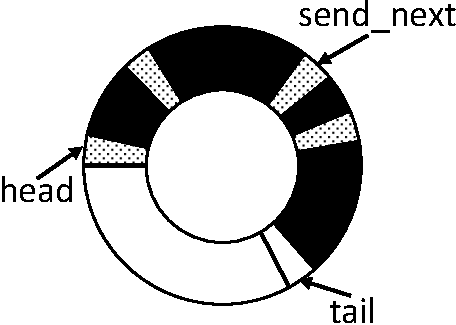
\includegraphics[width=0.32\textwidth]{images/ringbuffer_new}
		\label{socksdirect:fig:ringbuffer-new}
	}
	
	\caption{Ring buffer data structure. The shaded part is metadata, and the black part is the valid payload.}
\end{figure}


Traditionally, the network protocol stack uses a ring buffer to send and receive packets from the network card.
As shown in Figure \ref {socksdirect:fig:ringbuffer-traditional}, the traditional ring buffer consists of a set of fixed-length metadata, each of which points to a fixed-length memory page to store the valid payload. This design leads to memory allocation overhead and internal fragmentation.
The reason why traditional network cards use this design is that the number of ring buffers is limited, and multiple connections need to reuse a ring buffer. This design can move the metadata of the valid payload to the metadata queue of each connection without copying the content of the valid payload.
Fortunately, the one-sided RDMA write operation (write verb) opens up new design possibilities.
The innovation of this chapter is that \emph {each socket connection has its own dedicated ring buffer} and stores packets back-to-back, as shown in Figure \ref {socksdirect:fig:ringbuffer-new}.
The sender determines the offset in the ring buffer (i.e., the \emph{tail} pointer), and then uses a one-sided RDMA write operation to write the packet into the position pointed to by the \emph{tail} pointer in the remote memory.
During the transmission process, the receiving end CPU does not need to do anything.
When the receiving end application calls the \texttt {recv} operation, the data is dequeued from the position of the ring buffer pointed to by the \emph {head} pointer.
When the \emph{head} pointer moves to coincide with the \emph{tail}, the metadata pointed to by the pointer is empty, so the receiving end's \libipc{} library can detect that the queue is empty.
It should be noted that the \emph{head} and \emph{tail} pointers are maintained locally by the receiver and sender, respectively, so there is no need to synchronize these two pointers.
The process of transmitting data through shared memory is similar, because both shared memory and RDMA support write operations.



In order to judge whether the ring buffer is full, the sender will keep a \textit {queue credit} count, indicating the number of free bytes in the ring buffer.
When the sender enqueues a packet, it will consume credits equal to the size of the enqueued packet.
When the credits are insufficient, the sender will block and wait.
When the receiver dequeues the packet, it will increase the counter locally, and when the counter exceeds half of the size of the ring buffer, it will write a \textit {credit return flag} into the memory of the sender. The sender regains the queue credit when it detects this flag.
Please note that the queue credit mechanism is unrelated to congestion control; the latter is handled by the network card hardware \cite {zhu2015congestion}.

\textbf {Both the sender and receiver have a copy of the ring buffer.}
The above mechanism still requires the sender to allocate memory, because the sender needs a buffer to construct the RDMA message.
Secondly, the above mechanism does not support container hot migration, because the remaining data in the RDMA queue that has not been received in time is difficult to migrate.
Third, the goal of this chapter is to batch process small messages to improve throughput.
For this purpose, this chapter keeps a copy of the ring buffer at both the sender and receiver.
The sender writes to its local ring buffer and calls a one-sided RDMA write operation to synchronize the sender's ring buffer with the receiver's.
In order to minimize latency on idle links and maximize throughput on busy links, this paper designs an adaptive batching mechanism.
\libipc{} creates an RDMA reliable connection (RC) queue pair (QP) for each ring buffer and maintains a counter of RDMA messages.
If the counter does not exceed the threshold, an RDMA message is sent for each socket \texttt {send} operation.
Otherwise, the message is not sent temporarily, but the first unsent message is marked with \emph {send\_next}.
After completing the RDMA write operation, \libipc{} sends a message containing all unsent changes (from \emph {send\_next} to \emph {tail}) in Figure \ref {socksdirect:fig:ringbuffer-new}.
For shared memory, since cache coherence hardware can automatically perform inter-core synchronization, only one ring buffer shared by two processes is needed \footnote{Shared memory is a physical page mapped to the user address space of two processes respectively.}.

\textbf{Consistency between payload and metadata.}
For shared memory, Intel and AMD's x86 processors provide total store ordering \cite{sewell2010x86,intel-manual}, which means that each CPU core observes the write order of other CPU cores to be the same. The 8-byte \texttt{MOV} instruction is atomic, so writing the packet header is atomic. Since the sender writes the packet header after the payload, the message read by the receiver is consistent, and no memory barrier instruction is required.

Because RDMA cannot guarantee the write order of different parts of the message \cite{infiniband2000infiniband}, it is indeed necessary to ensure that the message is fully arrived before processing the message. Although the write of the message is always sequential in RDMA network cards using go-back-0 or go-back-N packet recovery~\cite{dragojevic2014farm}, this is not the case for more advanced network cards with selective retransmission \cite{mprdma,mittal2018retransmission}. In \libipc{}, the sender uses the RDMA \textit{write with immediate} operation to generate a completion event at the receiver. The receiver polls the RDMA \emph{completion queue} rather than the ring buffer. RDMA can ensure the cache consistency of the receiver and guarantee that the completion event is later than the data written to the \libipc{} ring buffer.

\textbf{Amortizing polling overhead.}
When sockets are not frequently used, polling the ring buffer wastes the receiver's CPU cycles. This chapter uses two techniques to amortize the polling overhead.
Firstly, for RDMA queues, the RDMA network card multiplexes event notifications into a single queue.
Each thread uses a \emph{shared completion queue} for all RDMA QPs, so it only needs to poll one queue instead of all socket queues.

Secondly, each queue can switch between \textit{polling} and \textit{interrupt} modes. The queue of the monitor is always in polling mode. The receiver of each queue maintains a counter for continuous empty polling. When it exceeds a threshold, the receiver sends a message to the sender, notifying that the queue is entering interrupt mode, and stops polling after a short time. When the sender writes to the queue in interrupt mode, it also notifies the monitor, and the monitor will notify the receiver to resume polling.

%\RED{Need a performance comparison figure of ring buffer architectures. (traditional ring buffer, new ring buffer, intra, inter, x axis: msg size, y axis: throughput)}

\subsection{Zero-copy}
\label{socksdirect:subsec:zerocopy}

The main challenge of zero-copy is to maintain the semantics of the socket API. Fortunately, virtual memory provides an indirect layer, and many related works have taken advantage of this \emph{page remapping} technique, which can remap physical pages from the sender's virtual address to the receiver's without copying. Linux zero-copy sockets \cite{linux-zero-copy} only support the sender, and they work by setting the data page to copy-on-write. However, many applications often overwrite the send buffer after calling \texttt{send}, so the copy-on-write mechanism only delays the copy from the time of calling \texttt{send} to the time of the first overwrite. To achieve zero-copy reception, 20 years ago, BSD~\cite{thadani1995efficient} and Solaris~\cite{chu1996zero} remapped the virtual pages of the application buffer to the physical pages of the operating system buffer. However, as shown in Table \ref{socksdirect:tab:operation-performance}, on modern CPUs, the cost of remapping a page is even higher than copying it due to kernel crossing and TLB refresh overhead. Recently, many high-performance TCP/IP stacks \cite{han2012megapipe,yasukata2016stackmap} and socket-to-RDMA libraries \cite{rsockets,socketsdirect} provide standard socket APIs and alternative zero-copy APIs, but they have not implemented zero-copy for the standard API. In addition, no existing work supports zero-copy for intra-host sockets.

%A sender may write the send buffer after non-blocking \texttt{send}, and the receiver does not know the receive buffer before \texttt{recv}.
% so we can remap virtual address of a buffer to another physical page if the data occupies entire 4~KiB pages.

To enable zero-copy, the network card driver needs to be modified to expose several kernel functions related to page remapping. To amortize the cost of page remapping, \libipc{} only uses zero-copy for \texttt{send} or \texttt{recv} if the payload is at least 16~KiB. Smaller messages are copied directly.

\textbf{Memory alignment.} Page remapping is only effective when the send and receive addresses are page-aligned and the transfer includes entire pages. \libipc{} intercepts \texttt{malloc} and \texttt{realloc} functions and allocates 4~KiB aligned addresses for memory allocation operations larger than 16~KiB, so most buffers will be aligned with page boundaries, and smaller memory allocations are allocated as before to avoid internal fragmentation. If the size of the sent message is not a multiple of 4~KiB, the last piece of data that is not a whole page will be copied during \texttt{send} and \texttt{recv}.

Sometimes, applications need to receive or send data not from the starting address of the allocated buffer. For example, the data is part of an HTTP request, the memory of the HTTP request is aligned, but the data is not aligned due to the presence of the HTTP header. For non-aligned cases, if the application sends directly after receiving without reading and writing the data itself, \sys{} can also achieve zero-copy message transmission. The method of \sys{} is that for non-aligned receive buffers, no memory copy is performed by default, but the mapping and offset relationship of the page is recorded. When the application accesses for the first time, the data copy is triggered by the page exception; if the application does not access the data, no copy is needed.

%\textbf{Amortize page remapping cost.}

\textbf{Reduce copy-on-write.} When the sender overwrites the buffer after \texttt{send}, the existing design uses copy-on-write. Copying is necessary because the sender may read the unwritten part of the page. Since applications almost always reuse the buffer for subsequent send operations, copy-on-write is called in most cases, making zero-copy basically useless for the sender. This paper observes that most applications do not write to the send buffer byte by byte. Instead, they overwrite the entire page of the send buffer through \texttt{recv} or \texttt{memcpy}, so there is no need to copy the original data of the page. For \texttt{memcpy}, \libipc{} calls the kernel to remap new pages and disable copy-on-write, and then performs the actual copy. For \texttt{recv}, the old page mapping is replaced by the received page.

\textbf{Page allocation overhead.}
The page remapping mechanism requires the kernel to allocate and release memory pages for each zero-copy \texttt{send} and \texttt{recv}.
Page allocation in the kernel uses a global lock, which is inefficient. Therefore, \libipc{} manages the available page pool in each process locally.
\libipc{} also tracks the source of the received zero-copy pages.
When a page is unmapped, if it comes from another process, \libipc{} returns the page to the owner through a message.

\begin{figure}[htbp]
	\centering
	\subfloat[Shared memory within the server. 1) Obtain physical pages and set write-on-copy; 2) Send page address via shared memory; 3) Map received pages; 4) (Optional) Remap during write / memcpy / recv on the sender side.]{
		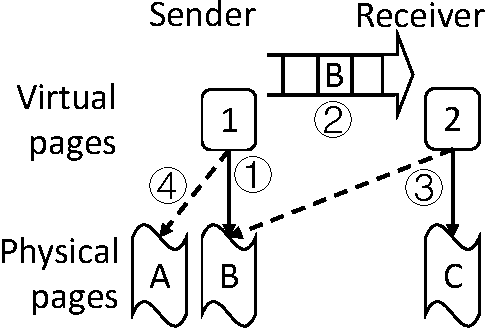
\includegraphics[width=0.44\textwidth]{images/zerocopy_intra}
		\label{socksdirect:fig:zerocopy-intra}
	}
	\hspace{0.02\textwidth}
	\subfloat[RDMA between servers. 1) Obtain physical pages and set write-on-copy; 2) Get available pages from the page pool; 3) Send data via RDMA; 4) Send page address via RDMA; 5) Map received pages; 6) Return unmapped pages to the page pool.]{
		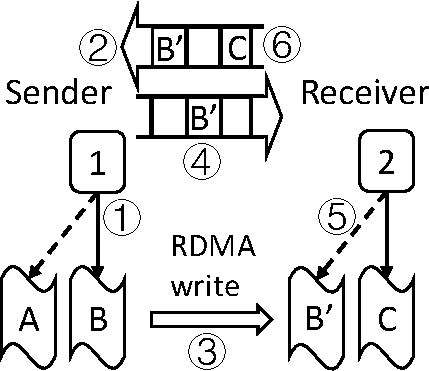
\includegraphics[width=0.42\textwidth]{images/zerocopy_inter}
		\label{socksdirect:fig:zerocopy-inter}
	}
	\caption{Process of sending zero-copy pages.}
\end{figure}

\textbf{Securely sending page addresses via shared memory.}
For intra-host sockets, \libipc{} sends physical page addresses in the user-space queue messages, as shown in step 2 of Figure \ref{socksdirect:fig:zerocopy-intra}.
For security, \sys{} must prevent arbitrary page mapping without the sender's permission.
To this end, \libipc{} calls the modified network card driver to get the encrypted physical page address of the send buffer and sends the encrypted address to the receiver via the shared memory queue.
On the receiver side, \libipc{} calls the kernel to remap the encrypted physical page address to the virtual address of the receive buffer provided by the application.

\textbf{Zero-copy under RDMA.}
\libipc{} initializes a fixed page pool on the receiver and sends the physical addresses of the pages to the sender.
The page pool is managed by the sender.
On the sender side, \libipc{} pins the virtual to physical page mapping of the send buffer, then allocates pages from the remote receiver's page pool to determine the remote address for RDMA write, as shown in step 2 of Figure \ref{socksdirect:fig:zerocopy-inter}.
On the receiver side, when \texttt{recv} is called, \libipc calls the network card driver to map the pages in the pool to the virtual address of the application buffer.
After the remapped pages are released (for example, they are overwritten by another \texttt{recv}), \libipc{} returns them to the page pool manager on the sender side (step 6).

\subsection{Event Notification}
\label{socksdirect:subsec:process-mux}

\textbf{Challenge 1: Multiplexing events between the kernel and \libipc{}.}
Applications poll for events from sockets and other \textit{kernel file descriptors} handled by the Linux kernel.
A simple way to poll for kernel events is to call a system call (such as \texttt{epoll\_wait}) each time, which incurs high overhead because event polling is a frequent operation that is almost called every time send and receive are called.
LOS~\cite{huang2017high} periodically calls the non-blocking \texttt{epoll\_wait} system call with kernel file descriptors, leading to a trade-off between latency and CPU overhead: if called too frequently, the CPU overhead is high; if not called frequently enough, the average latency of notifying kernel events to the application is high.
In contrast, \libipc{} creates an \textit{epoll thread} in each process, which calls the \texttt{epoll\_wait} system call to poll for kernel events. Whenever the epoll thread receives a kernel event, the application thread will report this event along with user-space socket events.

\textbf{Challenge 2: Interrupting busy processes.}
The socket takeover mechanism (Section \ref{socksdirect:subsubsec:fork_rdwr}) requires processes to respond to monitor requests. However, processes may execute application code for a long time without calling \libipc{}, and monitor requests cannot be responded to. To solve this problem, this chapter designs a \textit{signal} mechanism analogous to interrupts in the operating system. After the monitor sends a request, it first polls the receive queue for a while, and if there is no reply after a timeout, it sends a Linux \textit{signal} to wake up the corresponding process.

The signal handler registered by \libipc{} first determines whether the process is executing the application or the \libipc{} code. \libipc{} sets and clears flags at the entrance and exit of the library. If the signal handler finds that the process is in \libipc, it does nothing, and \libipc{} will handle the event before returning control to the application. Otherwise, the signal handler will immediately process the monitor's message.
Since \libipc{} is designed to be fast and non-blocking (all system calls that may cause blocking are called in the epoll thread), the monitor will receive a response quickly after sending the signal.

\textbf {Challenge 3: Let multiple threads share the core in time.}
For blocking socket operations (such as, blocking recv, connect and epoll\_wait), \libipc{} first polls the ring buffer once. If the operation is not completed, \libipc{} calls \textit {sched\_yield} to give up the CPU and switch to other processes on the same core. As described in Section \ref {socksdirect:subsec:motivation}, context switching in cooperative multitasking only requires 0.4~$\mu$s. However, some applications may need to wait a long time to receive a socket message, which leads to frequent wasteful awakenings. For this, \libipc{} counts the consecutive awakenings that do not process any messages, and puts the process to sleep when it reaches a threshold.
If the number of \libipc{} idling times reaches a certain threshold, it will put itself to sleep. Before going to sleep, it sends a message to the monitor and all processes (peers) that communicate directly with it, so that it can be awakened later by a signal.


\subsection{Connection Management}
\label{socksdirect:subsec:connection-management}

\subsubsection{File Descriptor Remapping Table}
\label{socksdirect:subsubsec:fd-remapping-table}

Socket file descriptors and other file descriptors (such as disk files) share a namespace, and Linux always allocates the smallest available file descriptor. To preserve this semantics without allocating virtual file descriptors in the kernel, \libipc{} intercepts all Linux APIs related to file descriptors and maintains a \emph{file descriptor remapping table} to map each application file descriptor to a user-space socket object or kernel file descriptor. When a file descriptor is closed, \libipc{} puts it into a \emph{file descriptor recycling pool}. When allocating a file descriptor, \libipc{} first tries to get a file descriptor from the pool. If the pool is empty, it allocates a new file descriptor by incrementing the \emph{file descriptor allocation counter}. The file descriptor recycling pool and allocation counter are shared among all threads in a process.

\subsubsection{Connection Establishment}

Figure \ref{socksdirect:fig:conn-setup} shows the connection establishment process.

\begin{figure}[htbp]
	\centering
	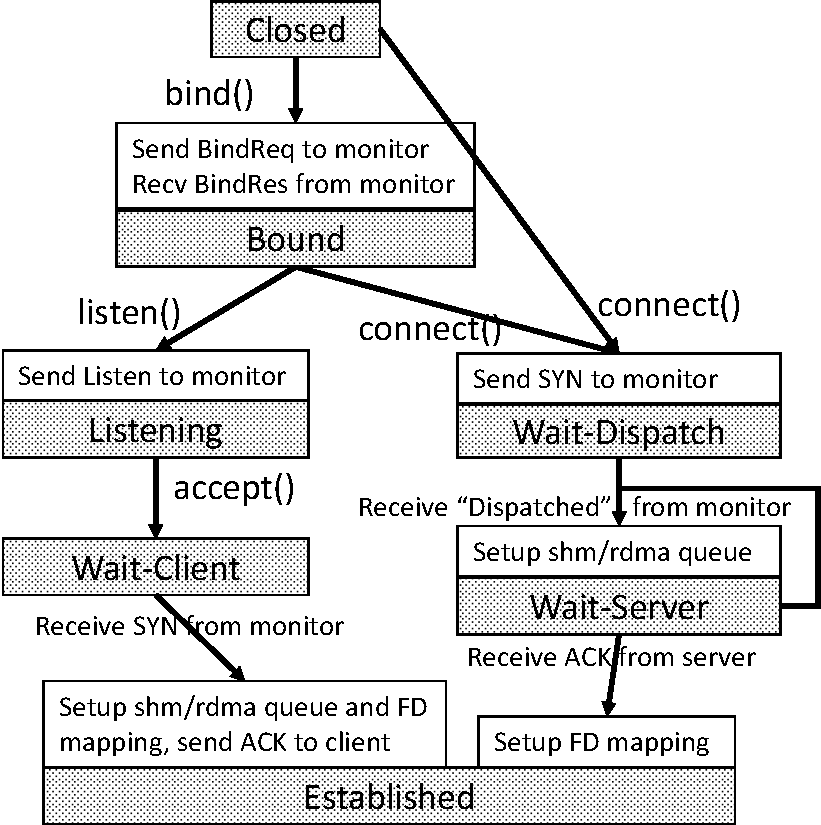
\includegraphics[width=0.6\textwidth]{images/conn-setup-new}
	\caption{State machine of the connection establishment process in \libipc{}.}
	\label{socksdirect:fig:conn-setup}
\end{figure}

\textbf{Binding Address (bind).} After creating a socket, the application calls \texttt{bind} to allocate an address and port. Since the address and port are globally protected resources, allocation is coordinated by the monitor. As shown in Figure \ref{socksdirect:fig:conn-setup}, \libipc{} sends the request to the monitor. To hide the latency of communicating with the monitor, as an optimization, if the bind request cannot fail (for example, when no port is specified for the client socket), \libipc{} immediately returns to the application.

\textbf{Listening Port (listen).} When the server application is ready to accept connections from clients, it calls \texttt{listen} and notifies the monitor. The monitor maintains a list of listening processes on each address and port to dispatch new connections.

\textbf{Initiating Connection (connect).} The client application calls \texttt{connect} and sends a SYN command to listen via the shared memory queue. Now, the monitor needs to dispatch the new connection to the listening application. In Linux, new connection requests are queued in the kernel's \emph{backlog}. Each time the server application calls \texttt{accept}, it accesses the kernel to dequeue from the backlog, which requires synchronization and increases latency. To solve this problem, \sys{} maintains a backlog for each listener thread of each listening socket. The monitor distributes the SYN to the listener threads in a round-robin manner.

When the listener does not accept new connections, connections dispatched to that listener may cause starvation. \sys{} uses a \emph{work stealing} method. When the listener calls \texttt{accept} when the backlog is empty, it requests the monitor to steal from others' backlogs. To avoid race conditions between the listener and the monitor, the monitor sends a request to the listener to steal from the backlog.

\textbf{Establishing Peer-to-Peer Queues.}
Upon the first communication between the client and server applications, the server monitor can assist them in establishing a direct connection. For within the host, the monitor allocates shared memory queues and sends the shared memory key to the client and server applications. For between hosts, the client and server monitors establish a new RDMA QP, and send the local and remote keys to the corresponding applications. To reduce latency, when the SYN command is dispatched to the backlog of the listener, the monitor establishes a peer-to-peer queue. However, if the SYN is stolen by another listener, a new queue needs to be established between the client and the new listener, as shown in the Wait-Server state in Figure \ref{socksdirect:fig:conn-setup}.

\textbf{Final Steps of Connection Establishment.}
After the server sets up the peer queue, as shown on the left side of Figure \ref{socksdirect:fig:conn-setup}, the server application sends an ACK to the client. The ACK contains the client file descriptor from the SYN request and its allocated server file descriptor. Similar to a TCP handshake, the server application can send data to the queue after sending the ACK. When the client receives the ACK, as shown on the right side of Figure \ref{socksdirect:fig:conn-setup}, it sets up the file descriptor mapping and can start sending data.

\subsubsection{Compatibility with Regular TCP/IP Peers}

To be compatible with peers that do not support \sys{} and RDMA, \sys{} needs to transparently detect \sys{} capabilities and fall back to regular TCP/IP when the peer does not support it. However, regular Linux sockets do not support adding special options to TCP SYN and ACK packets. Due to middleboxes and network reordering, using another port (like LibVMA~\cite{libvma} does) is also unreliable. For this, \libipc{} first uses a kernel raw socket to directly send SYN and ACK packets with special options, and if there are no special options, it falls back to kernel TCP/IP sockets.

On the client side, the monitor sends a TCP SYN packet with special options over the network. If the peer has \sys{} capabilities, its monitor will receive the special SYN and know that the client has \sys{} capabilities. Then, the server responds with a SYN + ACK with special options, including credentials for setting up the RDMA connection, so that the two monitors can communicate via RDMA later. If the client or server monitor discovers that the peer is a regular TCP/IP host, it will use Linux's TCP connection repair feature \cite{tcp-connection-repair} to create an established TCP connection in the kernel. Then the monitor sends the kernel file descriptor to the application via a Unix domain socket, and \libipc{} can use the kernel file descriptor for future socket operations.

A tricky issue is that received packets are delivered to both the raw socket and the kernel network protocol stack, at which point the kernel will reply with an RST packet because this connection does not exist in the kernel. To avoid this behavior, the monitor installs \emph{iptables} rules to filter out such outbound RST packets.

\subsubsection{Connection Closure}

When an application calls \texttt{close}, \libipc{} removes the file descriptor from the remapping table. However, the socket might still be useful because the file descriptor can be shared with other processes, and there might be unsent data in the buffer. \libipc{} keeps track of the reference count for each socket, incrementing it at fork and decrementing it at close. To ensure that unsent data has been sent to the peer, a handshake between the peers is needed during connection closure, similar to TCP close. Because sockets are bidirectional, \texttt{close} is equivalent to performing \texttt{shutdown} in both the send and receive directions. As shown in Figure \ref{socksdirect:fig:conn-close}, when an application closes one direction of a connection, it sends a \emph{shutdown message} to the peer. The peer responds with a shutdown message. When \libipc{} has received shutdown messages in both directions, it deletes the socket.

\begin{figure}[htbp]
	\centering
	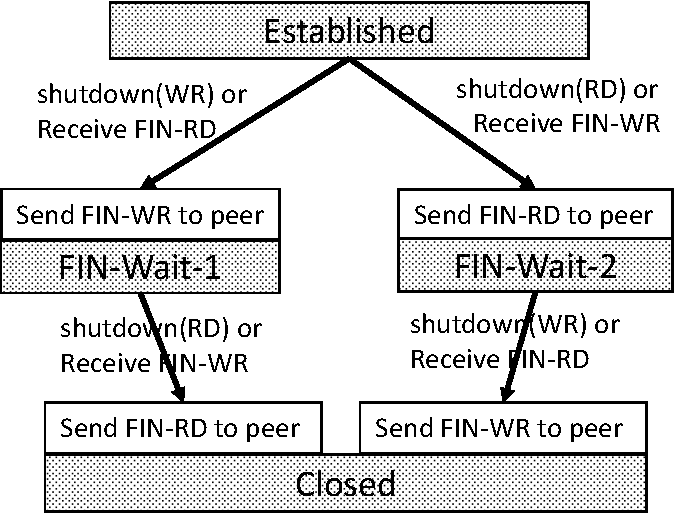
\includegraphics[width=0.5\textwidth]{images/conn-close-new}	
	\caption{State machine for connection closure in \libipc{}.}
	\label{socksdirect:fig:conn-close}
\end{figure}

\iffalse

\textbf{\texttt{Bind} and \texttt{listen}.}
A \emph{server} process \texttt{bind}s a socket and needs to detect IP and port conflict. In this case, \texttt{bind} is non-partitionable and goes to the monitor. The monitor also listens on the IP and port in a user-space TCP/IP stack (\textit{e.g.} mTCP~\cite{jeong2014mtcp}, LibVMA~\cite{libvma} or Seastar~\cite{seastar}) to receive connections from other hosts.

A \emph{client} process typically \texttt{bind}s without specifying IP and port, so we need to allocate a unique IP and port for it. For scalability, we partition the loopback IP address space (127.0.0.0/8) and each process allocates IP and port in its range.

\textbf{\texttt{Connect} and \texttt{accept}.}
When a client process connects to a server process on the same host, it sends a \textit{connect request} to the monitor via shared memory queue. When the server process is on another host, it creates a \textit{bootstrap TCP socket} with a special option via the user-space TCP/IP stack. If the server host supports the option, it is a \sys host and its monitor establishes an RDMA connection to the client to speedup later communications. Otherwise, the client process keeps using the bootstrap TCP socket for compatibility.

On a server host, the monitor distributes connect requests to server processes in a round-robin order, and a \textit{backlog} is maintained in each process. If the client is TCP only, the monitor proxies messages between the server process and the user-space TCP/IP stack. If the client is intra-server or RDMA capable, and it is the first time for the client and server processes to communicate, the monitor creates an inter-process queue for the process pair and sends the credentials to both processes via bootstrap sockets. After a server process \texttt{accept}s a connection in the backlog, it sends a message to the client via inter-process queue to create a file descriptor mapping, then the socket is ready for data transmission. As Figure~\ref{socksdirect:fig:conn-setup} shows, connection creation takes three inter-process delays.

Distributing connection to listeners may lead to starvation when a listener does not \texttt{accept} new connections. We devise a \textit{work stealing} approach. When a listener \texttt{accept}s from empty backlog, it requests the monitor to steal from others' backlog. To avoid polling empty backlogs, each listener notifies the monitor when its backlog becomes empty. To avoid contention between a listener and monitor, the monitor sends a request to the listener rather than stealing from the backlog directly.

%\subsubsection{Connection Close}

\textbf{\texttt{Close} and \texttt{shutdown}.}
Closing a connection is a peer-to-peer operation because only the peer process needs to be notified. If the file descriptor is deleted immediately after \texttt{close}, a new connection may reuse the file descriptor while the peer process might not yet have received the close event thus sends data to the wrong connection. To avoid this, we require a handshake between peers.
Because a socket is bidirectional, \texttt{close} is equivalent to \texttt{shutdown} on both send and receive directions.
When an application shuts down one direction of a connection, it sends a \textit{shutdown message} to the peer. The peer responds with a shutdown message. A process deletes a file descriptor when it receives shutdown messages in both directions.

%In order to achieve high scalability, we separate scalable operations to different processes. To avoid the overhead of contention, \libipc enable the file descriptor allocation by individual process and when a connection is setup, the other peer of the connection gets notified of the file descriptor number by message passing. Since we treat different threads in one process as different processes, we allocate file descriptor of different ranges to each of them to avoid collision. Since file descriptor is managed separately by each process, it is possible that a file descriptor is reused after the connection is closed. Our solution is that resources of a file descriptor is not released until an ACK is received for the close operation.

%Generally, each process in our design is treated as an endpoint in the network. Figure \ref{socksdirect:fig:conn-setup-close} shows the process of connection setup and close. When \textit{socket} is called, the process itself allocate per fd resources. When \textit{listen} is called, monitor is notified of port occupation. During the \textit{connect} operation, monitor first chooses one of the processes listen on this port then coordinates the creation of the shared memory between the two processes and notifies each other of the new connection. When \textit{close} happens, both of the endpoint notify each other and monitor is responsible to destroy the shared memory between them.

The LaTeX command "\fi" is not translatable as it is a part of the LaTeX markup structure. It is used to denote the end of an "if" statement in LaTeX. As per your instructions, I am not allowed to change the LaTeX markup structure. Therefore, the translated document remains the same:

\fi
